\section{Design}
\label{sec:design}

Figure~\ref{fig:architecture} summarizes the system boundary.  The sparse
flexible code matrix is fixed before an iteration, so the runtime does not
change which encoded rows or recovery sets exist.  \textsc{G-port} operates on
the worker-service path: it scores row pairs, predicts whether an adaptive
assignment will expose a decodable prefix earlier than static placement, runs a
fixed online guard, and then streams rows to TCP or K3s worker services.  The
exact row-span decoder remains the correctness gate, while the observed
first-decode event feeds the guard counters for later rounds.

\begin{figure*}[tbp]
  \centering
  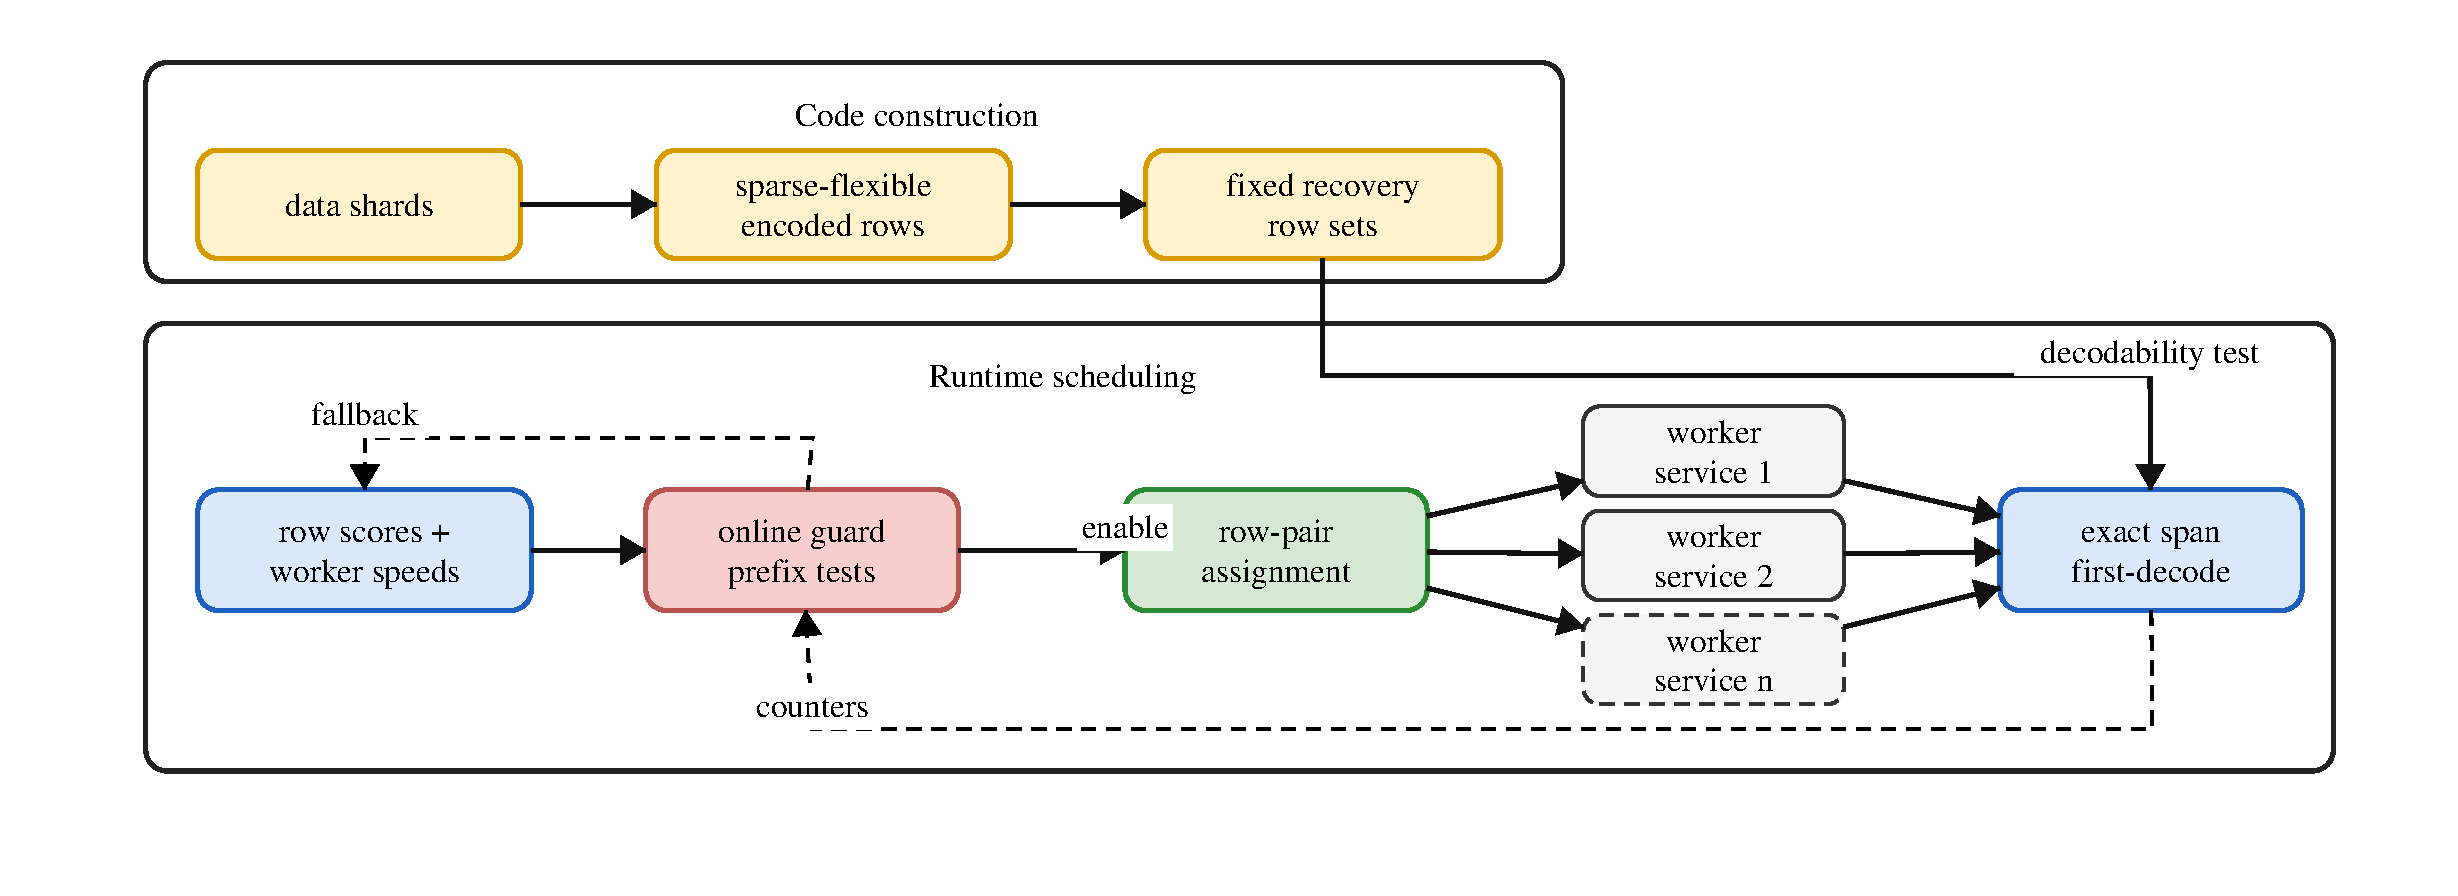
\includegraphics[width=\linewidth]{figures/figure1_architecture.pdf}
  \caption{Guarded first-decodable scheduling separates fixed code construction
  from runtime row exposure.}
  \Description{Two-lane architecture diagram. The top lane constructs fixed
  sparse-flexible encoded rows and recovery sets. The bottom lane uses row
  scores, worker speeds, an online guard, TCP worker services, and an exact
  first-decode monitor with counter feedback.}
  \label{fig:architecture}
\end{figure*}

\subsection{First-Decodable-Time Objective}

At iteration $t$, worker $j$ has a random completion time determined by its
current speed, queueing delay, and the sparse cost of the assigned row pair.
Let $\pi(i)$ denote the worker assigned to row pair $i$, containing rows $i$
and $i+n$ of the fixed code matrix $B$.  For a time $u$, let $S_\pi(u)$ be the
set of encoded rows completed by time $u$ under assignment $\pi$.

Under the exact row-span decoder used in this paper, the first decodable time is
\begin{equation}
  \label{eq:first-decodable-time}
  \tau(\pi, B) =
  \inf \{u : \mathbf{1}_m \in \mathrm{span}(B_{S_\pi(u)}^\top) \}.
\end{equation}
The system objective is
\begin{equation}
  \label{eq:first-decodable-objective}
  \min_\pi \mathbb{E}[\tau(\pi, B)].
\end{equation}

The objective in Equation~\eqref{eq:first-decodable-objective} differs from
minimizing total computation, assigned cost, or mean worker completion time.
It cares only about the earliest algebraically
sufficient set of returned rows.  The exact objective is combinatorial because
each completed subset has a different decodability status.  We therefore build
low-cost surrogates that preserve the central signal: how much a row
contributes to recovering the target vector $\mathbf{1}_m$.

\subsection{Target-Specific Decode Importance}

The scheduler needs a cheap signal for which encoded rows are useful for
recovering the target vector $\mathbf{1}_m$.  Let
$z\in\mathbb{R}^{2n}$ be a row-weight vector over all encoded rows of the fixed
code matrix $B$.  If every encoded gradient were available, coefficient $z_r$
would multiply the vector returned by row $r$.  The weighted sum recovers the
full gradient exactly when $B^\top z=\mathbf{1}_m$, because then the total
coefficient on every shard gradient is one.  Among all row-weight vectors that
satisfy this recovery condition, we choose the minimum-norm reference decoder
\begin{equation}
  \label{eq:reference-decoder}
  z^\star =
  \arg\min_z \|z\|_2^2
  \quad \mathrm{s.t.} \quad
  B^\top z = \mathbf{1}_m .
\end{equation}
When the target vector is recoverable from the full code matrix, this reference
decoder has the closed form
\begin{equation}
  \label{eq:reference-decoder-closed}
  z^\star = B(B^\top B)^\dagger \mathbf{1}_m .
\end{equation}
Equations~\eqref{eq:reference-decoder}
and~\eqref{eq:reference-decoder-closed} are computed only from the fixed code
matrix and the target full-gradient vector.  Here $(\cdot)^\dagger$ is the
Moore--Penrose pseudoinverse.  The vector
$z^\star$ is not the online decoder used after partial results arrive; online
decoding still solves the exact row-span condition on the returned subset.  We
use $z^\star$ only as a pre-runtime signal: if row $r$ has a large coefficient
in this reference decoder, delaying that row is more likely to delay a recovery
path for $\mathbf{1}_m$.  We therefore define the target-specific importance of
row $r$ as
\begin{equation}
  \label{eq:row-importance}
  \rho_r = |z^\star_r|.
\end{equation}

The runtime assigns row pairs rather than individual rows.  Pair $i$ contains
rows $i$ and $i+n$, and its sparse computation cost is $C_i$.  The scheduler
uses the pair priority
\begin{equation}
  \label{eq:pair-priority}
  R_i = (\rho_i + \rho_{i+n}) C_i,
\end{equation}
so a pair becomes high priority only when it is both decode-relevant and costly
enough for placement to matter.  Equation~\eqref{eq:pair-priority} is a
scheduling feature, not a
recovery certificate.  The runtime still accepts decoding only after the exact
row-span test succeeds on streamed completions.  Multiplying by $C_i$ is a
systems choice rather than a theorem: a high-$\rho$ row with negligible cost
does not need a scarce early worker, while a costly row matters only if it is
also decode-relevant.  The evaluation therefore treats score variants as
diagnostics, and the guard remains the protection against regimes where this
feature is misaligned with true first-decode criticality.

\subsection{Decode-Aware Assignment}

The decode-aware scheduler sorts row pairs by decreasing $R_i$ and workers by
decreasing estimated speed, then assigns the $k$th highest-priority row pair to
the $k$th fastest worker.  This simple monotone rule requires only the code
matrix and a current speed estimate.  It is
implemented as \textsc{RankAwareSparseFlexible} in the prototype.
The rule is deliberately conservative: it does not change the code, the number
of encoded rows, or the algebraic recovery condition.  It only permutes the
mapping between already-defined row pairs and available workers.

Algorithm~\ref{alg:decode-aware} shows the full scheduling path.  Lines 1--4
compute a target-specific decode-mass signal from the fixed code matrix.
Lines 5--7 lift that row-level signal to row pairs and multiply it by sparse
row-pair cost, because a high-importance row pair only changes wall-clock time
when its computation is nontrivial.  Lines 8--12 then perform the monotone
placement.  The important point is that $R_i$ is not treated as an independent
utility score for a completed row.  It is a proxy for how much delaying that
row pair can delay the first completed set whose span contains
$\mathbf{1}_m$.  Thus the scheduler tries to make the likely early prefix of
completed rows more decodable, rather than merely cheaper or faster in total.

\begin{algorithm}[t]
  \caption{Decode-aware row-pair assignment}
  \label{alg:decode-aware}
  \begin{algorithmic}[1]
    \Require Fixed code matrix $B$, pair costs $\{C_i\}$, worker speed estimates $\{s_j\}$
    \Ensure Row-pair to worker assignment $\pi$
    \State Compute $z^\star = B(B^\top B)^\dagger \mathbf{1}_m$
    \ForAll{encoded rows $r$}
      \State $\rho_r \gets |z^\star_r|$
    \EndFor
    \ForAll{row pairs $i$}
      \State $R_i \gets (\rho_i + \rho_{i+n}) C_i$
    \EndFor
    \State $(i_1,\ldots,i_n) \gets$ row pairs sorted by decreasing $R_i$
    \State $(j_1,\ldots,j_n) \gets$ workers sorted by decreasing $s_j$
    \For{$k=1,\ldots,n$}
      \State $\pi(i_k) \gets j_k$
    \EndFor
    \State \Return $\pi$
  \end{algorithmic}
\end{algorithm}

\subsection{Deadline-Aware Extension}

Decode-aware sorting is the main instantiation of the scheduling idea.  As a
stress-test extension for runtimes with transient delay, we also define a
deadline-aware matching score.  Let
\begin{equation}
  \label{eq:deadline-time}
  \widehat{T}_{ij} = d_j + \gamma C_i / s_j
\end{equation}
be the nominal completion time of pair $i$ on worker $j$, with delay $d_j$,
speed $s_j$, and runtime scale $\gamma$.  For a target deadline $q$, define the soft
completion probability
\begin{equation}
  \label{eq:deadline-probability}
  P_{ij}(q) = \exp(-\widehat{T}_{ij}/q).
\end{equation}
The scheduler solves
\begin{equation}
  \label{eq:deadline-assignment}
  \max_\pi \sum_i R_i P_{i,\pi(i)}(q),
\end{equation}
a standard linear assignment problem.  Equations~\eqref{eq:deadline-time},
\eqref{eq:deadline-probability}, and~\eqref{eq:deadline-assignment} define the
optional deadline-aware policy.  It builds
$W_{ij}=R_iP_{ij}(q)$ and calls \textsc{MaxWeightMatching}$(W)$, which returns
the assignment $\pi$ maximizing $\sum_i W_{i,\pi(i)}$.  In the current
prototype, $q$ is the median nominal completion time in the iteration.  The
extension is useful when transient delay makes the fastest worker by compute
speed differ from the earliest worker by response time.

\begin{algorithm}[t]
  \caption{Deadline-aware row-pair assignment}
  \label{alg:deadline-aware}
  \begin{algorithmic}[1]
    \Require Pair scores $\{R_i\}$, costs $\{C_i\}$, speeds $\{s_j\}$, delays $\{d_j\}$, deadline $q$
    \Ensure Row-pair to worker assignment $\pi$
    \ForAll{row pairs $i$ and workers $j$}
      \State $\widehat{T}_{ij} \gets d_j + \gamma C_i / s_j$
      \State $P_{ij}(q) \gets \exp(-\widehat{T}_{ij}/q)$
      \State $W_{ij} \gets R_i P_{ij}(q)$
    \EndFor
    \State $\pi \gets \Call{MaxWeightMatching}{W}$ \Comment{maximize $\sum_i W_{i,\pi(i)}$}
    \State \Return $\pi$
  \end{algorithmic}
\end{algorithm}

Algorithm~\ref{alg:decode-aware} requires one target-decoder computation when
the code changes and an $O(n\log n)$ sort per scheduling round.  The optional
deadline-aware variant adds an $n\times n$ weight matrix and a cubic-time exact
assignment solve.  It is therefore a stress-test policy, not the default path;
larger deployments can use the monotone sort, top-$k$ candidate matching, or
incremental rematching when few delay estimates change.

\subsection{Guard Enablement Conditions}

The scheduler is intentionally conditional: it is not expected to improve every
iteration.  It helps when two conditions hold.  First, static placement must be
misaligned with decode priority, so high-$R_i$ row pairs are not already on
workers likely to complete early.  Second, the reassignment must reduce the
arrival index of the first decodable set, or at least avoid increasing it by
more than the speedup can compensate.  In the prototype we expose this
through runtime counters for selected rows, completed rows, extra compute, and
scheduler time.  These counters are used in the evaluation to explain the
boundary between strong tail improvements and modest or negative gains.

This yields a fixed counter guard: enable adaptive assignment only when
estimated mismatch is positive and recent first-decode counters do not show a
larger completed-row prefix.  A payload $P=(B,\pi)$ combines the fixed code
matrix with a row-to-worker assignment.  \textsc{G-port}, the main system,
compares a safe fallback payload $P_0$ against candidate payloads and runs an
adaptive candidate only if every guard test passes.  Its
first-decode-aware coded
candidate is built by applying the row-pair scores from
Algorithm~\ref{alg:decode-aware} inside the deadline-aware matching of
Algorithm~\ref{alg:deadline-aware}; we call this coded candidate
\textsc{Guard-D}.  If the guard does not pass,
\textsc{G-port} falls back to static sparse-flexible placement.  Rank-only
ordering (\textsc{Guard-R}), coded-only \textsc{Guard-D}, and alternative
fallback choices are retained as ablations to isolate which part of the system
matters; they are not separate proposed methods.

Algorithm~\ref{alg:counter-guard} is the online guard used by the implemented
runtimes and replayed unchanged in diagnostic experiments.  In simulation and
replay studies, the rule is applied to recorded or synthesized worker states;
in multi-process and worker-service runs (TCP, Docker, and K3s), the master
executes it before each iteration.  The rule has four tests.  It first predicts
the static fallback
payload $P_0$ and the candidate coded payload $P_c$, then enables $P_c$ only
when worker speeds are heterogeneous enough, the predicted first-decode time is
lower, the predicted first-decode prefix does not grow, and recent monitored
counters do not show extra prefix growth or post-decode work.  Here
$\mathrm{cv}(\text{speed})$ is the coefficient of variation of the current
worker-speed estimates.  Thus the
decision is made before the iteration and cannot select a policy after seeing
that iteration's latency.

The counter update is conservative.  In cold start, the exponential
moving-average counters are zero, so the guard is controlled only by the current
worker state and the predicted static-vs-candidate prefix comparison.  After an
enabled round, the monitor updates the counters from the observed first-decode
event.  After a fallback round, the candidate did not run, so the counters decay
toward zero rather than being updated from the fallback's outcome.

\textsc{Predict} is an online model over current runtime features, not a replay
oracle.  For a payload $P=(B,\pi)$, it returns
$(\widehat{\tau},\widehat{K})$, where $\widehat{\tau}$ is predicted first-decode
time and $\widehat{K}$ is the predicted first-decodable prefix length.  Row $r$
assigned to worker $j=\pi(r)$ has nominal service time
\begin{equation}
  \label{eq:nominal-service}
  \widehat{x}_{rj}
  =
  \beta_d d_j + \beta_c c_r / \max(s_j,\epsilon),
\end{equation}
where $d_j$ and $s_j$ are the current delay and speed estimates, $c_r$ is row
cost, and $\beta_d,\beta_c$ are runtime scales.  If a worker receives multiple
rows, predicted completion is cumulative over its local queue:
\begin{equation}
  \label{eq:predicted-completion}
  \widehat{t}_r
  =
  \sum_{r' \preceq_j r} \max(0,\widehat{x}_{r'j}) .
\end{equation}
Here $r'\preceq_j r$ means row $r'$ is no later than $r$ in worker $j$'s queue.
Equations~\eqref{eq:nominal-service} and~\eqref{eq:predicted-completion}
therefore convert a payload into a predicted row-arrival order.
The predictor sorts rows by $\widehat{t}_r$ and runs the same incremental
row-span test as the decoder; the first successful arrival time is
$\widehat{\tau}$, and the successful prefix size is $\widehat{K}$.  Prediction
errors are handled conservatively by requiring positive predicted gain,
non-increasing predicted prefix, and non-growing EMA prefix counters before
enabling the candidate scheduler.

\begin{algorithm}[t]
  \caption{Online counter guard}
  \label{alg:counter-guard}
  \begin{algorithmic}[1]
    \Require Fallback payload $P_0$, candidate payload $P_c$, worker state,
      thresholds $\theta_{\mathrm{cv}},\theta_g,\theta_K,\theta_a$,
      EMA counters $\bar{\Delta K}$ and $\bar{A}$, update weight $\alpha_{\mathrm{ema}}$,
      fallback decay $\lambda$
    \Ensure Payload for this iteration and updated guard state
    \State Predict $(\hat{\tau}_0,\hat{K}_0)$ for $P_0$
    \State Predict $(\hat{\tau}_c,\hat{K}_c)$ for $P_c$
    \State $g \gets (\hat{\tau}_0-\hat{\tau}_c)/\hat{\tau}_0$
    \State $\Delta \hat{K}\gets \hat{K}_c-\hat{K}_0$
    \State $h\gets(\bar{\Delta K}\le\theta_K)\wedge(\bar{A}\le\theta_a)$
    \If{$\mathrm{cv}(\text{speed})\ge\theta_{\mathrm{cv}}$
        and $g\ge\theta_g$ and $\Delta\hat{K}\le\theta_K$ and $h$}
      \State run candidate scheduler $P_c$
      \State observe first-decodable prefix $K_c$ and rows-after-decode $A$
      \State $\bar{\Delta K}\gets(1-\alpha_{\mathrm{ema}})\bar{\Delta K}+\alpha_{\mathrm{ema}}(K_c-\hat{K}_0)$
      \State $\bar{A}\gets(1-\alpha_{\mathrm{ema}})\bar{A}+\alpha_{\mathrm{ema}} A$
    \Else
      \State run fallback $P_0$
      \State $\bar{\Delta K}\gets\lambda\bar{\Delta K}$; $\bar{A}\gets\lambda\bar{A}$
    \EndIf
  \end{algorithmic}
\end{algorithm}
